\section{Packet Error Probability}\label{sec:pep}
Now that we are able to simulate the \gls{rssi} when transmitting from one node to another, we need to be able to simulate whether the packet should arrive on the receiving node. With wireless radio communication, there is a chance that a receiving node may not receive the entire packet correctly, which is why we need some way of computing the probability of this happening. For this, we introduce the packet error probability. The computations in this section are derived from \cite{massoud2007digital}, as well as personal communication with the author of \cite{paper:linkmodel}. \medbreak

\subsection{Radio Model}

First we calculate the noise power $P_{N,db} = thermal\_noise + noise\_figure$ in \acrshort{db}. The noise power is calculated with the thermal noise and noise figure, and is the level of background noise affecting the wireless radio communication. For the Reachi devices we assume the $thermal\_noise = -119.66$ \acrshort{db} and the $noise\_figure = 4.2$ \acrshort{db}. \medbreak

Next we need to add the noise from interfering transmissions happening at the same time. We do this by adding the sum of the \gls{rssi} from interfering transmitters to the noise power $P_{N,dB}$, giving us $P_{NI,dB}$ on the link between the receiving node $n_r$ and the transmitting node $m_t$: 
\begin{eq}\label{eq:noisepower}
    P_{NI,db}(n_r, m_t) = 10 \log_{10}\left( 10^{\frac{P_{N,dB}}{10}} + \mathlarger{\sum}\limits_{m \in nodes_t}  10^{\frac{RSSI_{dBm}(n_{r}, m)}{10}} [m \neq m_{t}] \right) 
\end{eq}

The set of currently transmitting nodes are denoted by $nodes_t$ and the function $RSSI(n, m)$ denotes the RSSI on the link between nodes $n$ and $m$.\smallbreak

Next we calculate the signal to noise (and interference) ratio $\gamma_{dB}$ in \acrshort{db}. The ratio $\gamma_{dB}$ is the ratio between signal and noise, that compares the level of the signal to the level of the background noise (including the interference from other transmissions), and is computed by subtracting the noise power $P_{NI,db}$:

%We expand upon this further to include the interference of other transmissions happening at the same time. This is done by computing the \gls{rssi} from interfering transmitters, and subtracting this from the \gls{sinr}, which gives us the \acrlong{snir}:

% n receiver, m transmitter

%where we assume that the $thermal\_noise = -119.66$ \acrshort{db} and the $noise\_figure = 4.2$ \acrshort{db}.

%\begin{eq}
%    P_{N,db} = thermal\_noise + noise\_figure
%\end{eq}

%Signal to noise ratio with interference, on a link from $n_r$ (receiver) to $n_t$ (transmitter). The set of currently transmitting nodes are denoted by $nodes_t$. The function $RSSI(n, m)$ denotes the RSSI on the link between nodes $n$ and $m$. We subtract the sum of the RSSI between $n_r$ and any currently transmitting nodes, excluding $m_t$.

\begin{eq}
    \gamma_{dB}(n_r, m_t) = RSSI(n_r, m_t) - P_{NI,dB}(n_r, m_t)
\end{eq}

We use this to compute the bit error probability $P_b$:

%\begin{eq}
%    \gamma = 10^{\frac{\gamma_{dB}}{10}}
%\end{eq}

\begin{eq}
    P_b(n_r, m_t) = \frac{1}{2}erfc \left( \sqrt{ \left( \frac{10^{\frac{\gamma_{dB}(n_r, m_t)}{10}}}{2} \right)} \right)
\end{eq}

which we finally can use to compute the packet error probability $P_p$. The packet error probability is the probability that we experience a bit error for any of the bits in our packet, during transmission.

%\begin{eq}
%    P_b = \frac{1}{2}erfc \left( \sqrt{ \left( \frac{\gamma}{2} \right)} \right)
%\end{eq}

\begin{eq}
    P_p(n_r, m_t) = 1 - \left( 1 - P_b(n_r, m_t) \right) ^{packetsize}
\end{eq}

%\begin{figure}[ht]
%    \centering
%    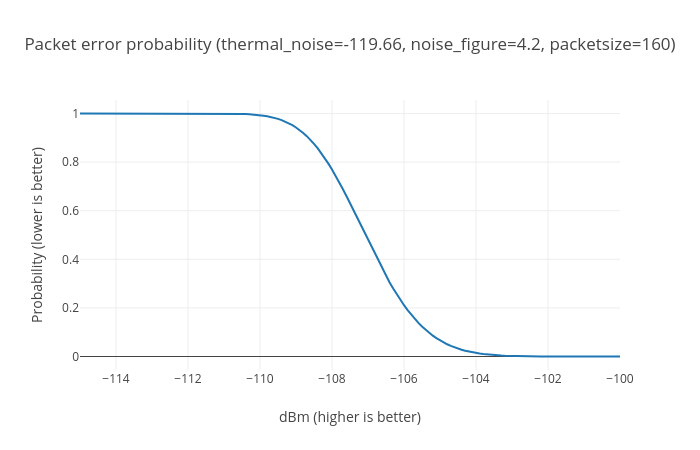
\includegraphics[width=.7\textwidth]{figures/pep/pep.png}
%    \caption{Limits.}
%    \label{figure:pepegraph}
%\end{figure}

\subsection{Example}
In \autoref{sec:linkmodel}, we computed the link model for a sample network topology \textbf{G}. \autoref{eq:rssivector} shows a vector containing the \gls{rssi}, in \acrshort{dbm}, for each of the six links in the network, assuming a transmission power of 26 \acrshort{dbm}. For the following, it is assumed that $thermal\_noise = -119.66$ \acrshort{db}, the $noise\_figure = 4.2$ \acrshort{db}, and $packetsize = 160$.

\begin{eq}\label{eq:rssivector}
    \vect{RSSI_{dBm, \textbf{G}}} = 
        \begin{bmatrix}
            -64.610\\
            -61.734\\
            -72.170\\
            -52.163\\
            -74.042\\
            -72.413
        \end{bmatrix}
\end{eq}

If we assume that $n_2$ is currently listening, and the currently transmitting nodes $nodes_t = {n_1, n_3, n_4}$. What is the probability for packet error on the link between nodes $n_2$ and $n_4$ with interference from nodes $n_1$ and $n_3$? First, we compute the noise power $P_{NI,db}$, according to \autoref{eq:noisepower}:

%\begin{eq}
%    P_{NI,db}(n_2, n_4) = 10 \log_{10}\left( 10^{\frac{(-119.66 + 4.2)}{10}} + \mathlarger{\sum}\limits_{m \in {n_1, n_3, n_4}}  10^{\frac{RSSI_{dBm}(n_{2}, m)}{10}} [m \neq n_{4}] \right) 
%\end{eq}

\begin{eq}
    P_{NI,db}(n_2, n_4) = 10 \log_{10}\left( 10^{\frac{(-119.66 + 4.2)}{10}} + 10^{\frac{-64.610}{10}} + 10^{\frac{-52.163}{10}}  \right) = -51.923
    %\mathlarger{\sum}\limits_{m \in {n_1, n_3}}  10^{\frac{RSSI_{dBm}(n_{2}, m)}{10}} [m \neq n_{4}] \right) 
\end{eq}

We subtract the noise power $P_{NI,db}$ from the \gls{rssi} to get the signal to noise (and interference) ratio $\gamma_{dB}$:

\begin{eq}
    \gamma_{dB}(n_2, n_4) = -74.042 - (-51.923) = -22.119
\end{eq}

With which we can compute the bit error probability:

\begin{eq}
    P_b(n_2, n_4) = \frac{1}{2}erfc \left( \sqrt{ \left( \frac{10^{\frac{-22.119}{10}}}{2} \right)} \right) = 0.469
\end{eq}

Finally we can compute the packet error probability using the bit error probability:

\begin{eq}
    P_p(n_2, n_4) = 1 - \left( 1 - 0.469 \right) ^{160} = 1.0
\end{eq}

With a probability for bit errors of approximately 47 \%, we can say with 100 \% probability that we will experience packet loss on the link from $n_2$ to $n_4$, with two interfering transmitters.



%If we assume that $n_2$ is currently listening, and the currently transmitting nodes are $nodes_t = {n_1, n_3, n_4}$. Now, we want to compute the probability for packet error on the link between nodes $n_2$ and $n_4$.

%\subsection*{Example}
%
%\begin{figure}[H]
%    \centering
%    \begin{tikzpicture}
%        \begin{scope}[xshift=4cm]
%        \node[main node] (1) {$1$};
%        \node[main node] (2) [left = 2cm  of 1]  {$2$};
%        \node[main node] (3) [below = 2cm  of 2] {$3$};
%        \node[main node] (4) [right = 2cm  of 3] {$4$};
%
%        \path[draw,thick]
%        (1) edge node[above] {$l_1$} (2)
%        (1) edge node[above=.8cm, right] {$l_2$} (3)
%        (1) edge node[right] {$l_3$} (4)
%        (2) edge node[left] {$l_4$} (3)
%        (2) edge node[below=.8cm, right] {$l_5$} (4)
%        (3) edge node[below] {$l_6$} (4)
%        ;
%        \end{scope}
%    \end{tikzpicture}
%    \caption{Sample graph \textbf{G} with 4 nodes and 6 links.}
%    \label{figure:lm-sample}
%\end{figure}
%

%The vector \vect{RSSI_{\textbf{G}}} contains the RSSI for all links in \textbf{G}. It is assumed that $thermal\_noise = -119.66$ \acrshort{db}, the $noise\_figure = 4.2$ \acrshort{db}, and $packetsize = 160$. \medbreak

%If we assume that $n_2$ is currently listening, and the currently transmitting nodes are $nodes_t = {n_1, n_3, n_4}$. Now, we want to compute the probability for packet error on the link between nodes $n_2$ and $n_4$.
%(-119.66 + 4.2)
%\begin{eq}
%    \gamma_{dB}(n_2, n_4) = RSSI(n_2, n_4) - P_{N,dB} - \mathlarger{\sum}\limits_{m \in \{n_1, n_3, n_4\}} RSSI(n_2, m)[m \neq n_4]
%\end{eq}
%
%\begin{eq}
%    \gamma_{dB}(n_2, n_4) = -74.042 - (-119.66 + 4.2) - (-64.610 + (-52.163)) = 158.191
%\end{eq}
%
%\begin{eq}
%    P_b(n_2, n_4) = \frac{1}{2}erfc \left( \sqrt{ \left( \frac{10^{\frac{158.191}{10}}}{2} \right)} \right) = 1.406 %\cdot 10^{-36}
%\end{eq}
%
%\begin{eq}
%    P_p(n_2, n_4) = 1 - \left( 1 - P_b(n_2, n_4) \right) ^{160} = 0.0
%\end{eq}

%Which equals to a probability of approximately 10 \% packet loss, with no interference, and an \gls{rssi} of $-105.3$ \acrshort{dbm}.
